\chapter{Project Gantt Chart}
\label{appendix:ganttChart}

\begin{ganttchart}[
  hgrid,
  vgrid,
  today=23,
  today rule/.style=%
    {draw=blue, ultra thick}
  ]{1}{23}

  % Titles
  \gantttitle{Semester 1}{12}
  \gantttitle{Semester 2}{11} \\
  \gantttitlelist{1,...,12}{1}
  \gantttitlelist{1,...,11}{1} \\

  % Groups
  \ganttgroup{Seminar}{8}{8} \\
  \ganttgroup{Presentation of results}{18}{20} \\

  % Deadlines
  \ganttmilestone{Code freeze/submission}{19} \\
  \ganttmilestone{Project showcase}{21} \\
  \ganttmilestone{Final report deadline}{23} \\

  % Bars
  \ganttbar{Project plan}{1}{1} \\
  \ganttbar{Research}{2}{6} \\
  \ganttbar{Language Learning}{4}{6} \\
  \ganttbar{Seminar prep}{5}{7} \\
  \ganttbar{First code sprint}{7}{11} \\
  \ganttbar{First retrospective}{12}{12} \\
  \ganttbar{Second code sprint}{13}{17} \\
  \ganttbar{Presentation preparation}{15}{17} \\
  \ganttbar{Bug bash/second retrospective}{18}{19} \\

  \ganttbar{Video creation}{20}{23} \\
  \ganttbar{Report writing}{2}{23}

\end{ganttchart}

\chapter{Queue Code}
\label{appendix:queueCode}

\inputminted[breaklines=true, breakanywhere]{go}{code/gamq/queue/queue.go}

\chapter{UdpWriter}
\label{appendix:udpWriter}

\inputminted[breaklines=true, breakanywhere]{go}{code/gamq/udp/udpwriter.go}

\chapter{Parse Client Command}
\label{appendix:parseClientCommand}

\inputminted[breaklines=true, breakanywhere, firstline=226, lastline=260]{go}{code/gamq/connectionmanager.go}

\chapter{Send Messages To Client}
\label{appendix:sendMessagesToClient}

\inputminted[breaklines=true, breakanywhere, firstline=35, lastline=67]{go}{code/gamq/messageshipper.go}

\chapter{Benchmark Code}
\label{chap:benchmarkCode}

\inputminted[breaklines]{python}{code/gamq/tools/benchmark/benchmark.py}

\chapter{Test Output}
\label{chap:testOutput}

\inputminted[breaklines]{bash}{code/goTestOutput}

\chapter{Test Output}
\label{chap:testOutput}
[see following page]
\begin{landscape}
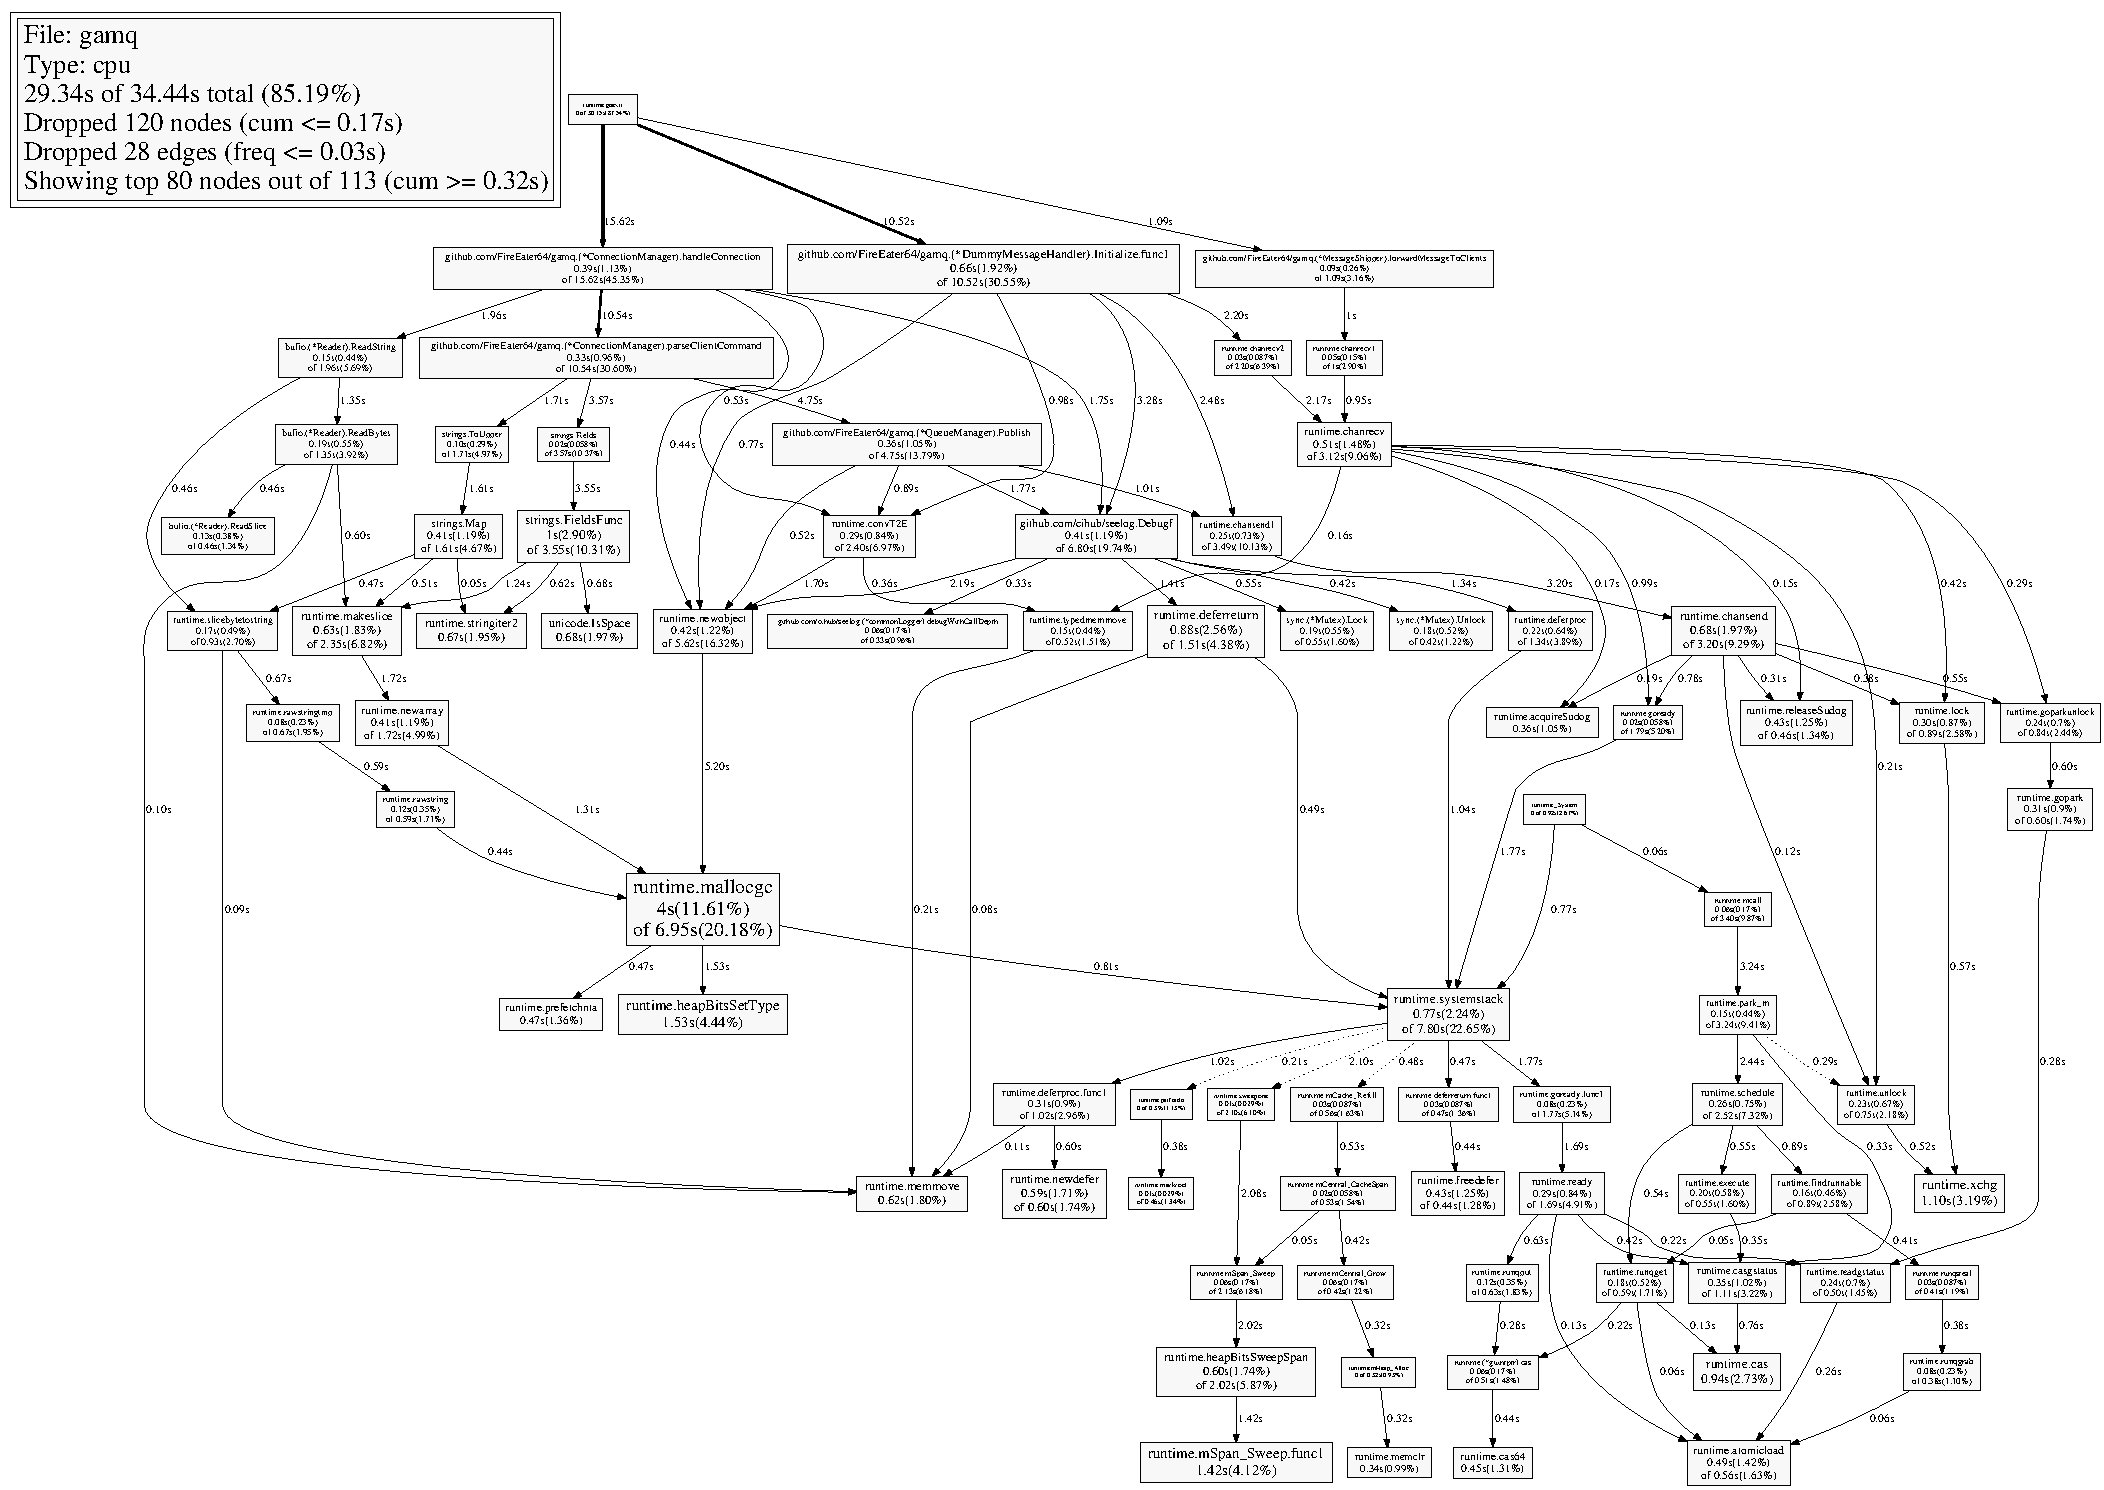
\includegraphics[width=\textwidth]{figures/profileOutput}
\end{landscape}
